\documentclass[landscape]{a0poster}

% Packages
\usepackage{aas_macros}
\usepackage{amsmath}
\usepackage{amssymb}
\usepackage{fontspec}
\usepackage{natbib}
\usepackage{graphicx}
\usepackage{xcolor}
\usepackage{lettrine}
\usepackage{flowfram}
\usepackage{url}
\usepackage{tikz}
\usetikzlibrary{calc,matrix,shapes.geometric,shapes.misc,shapes.symbols}

% Macros
\newcommand{\EM}[1]{\ensuremath{\textsc{\textrm{em}}_#1}}
\newcommand{\GW}{\ensuremath{\textsc{\textrm{gw}}}}
\newcommand{\dropcap}[2]{\lettrine{\fontspec{Copse}#1}{\textnormal{ #2}}}

% Adjust section style
\makeatletter
\renewcommand{\section}{\@startsection
{section}%                   % the name
{1}%                         % the level
{0mm}%                       % the indent
{-\baselineskip}%            % the before skip
{0.5\baselineskip}%          % the after skip
{\fontspec{Marvel Bold}\Huge}} % the style
\makeatother

% Adjust journal abbreviation style for AAS journal macros
\makeatletter
\let\jnl@style=\sf
\makeatother

% Adjust default font
\setsansfont[Mapping=tex-text]{Corbel}
\renewcommand{\familydefault}{\sfdefault}

% Adjust style for emphasized text
\renewcommand{\emph}[1]{{\bfseries\itshape#1}}

% Expand space between lines
\linespread{1.2}

% Increase paragraph indentation
\setlength{\parindent}{4em}

% Static frames
\newstaticframe{\textwidth}{0.3\textheight}{-0.125\textwidth}{0.81\textheight}[title-drawing]
\newstaticframe{28cm}{21cm}{4cm}{26cm}[efficiency_distance]
\newstaticframe{28cm}{21cm}{32cm}{26cm}[efficiency_histogram]
\newstaticframe{27cm}{20cm}{32cm}{0cm}[convergence]
\newstaticframe{16cm}{18cm}{48cm}{66cm}[healpix-dots]
\newstaticframe{27cm}{80cm}{88cm}{20cm}[flowchart]
\newstaticframe{40cm}{5cm}{32cm}{20cm}[ligosmile]
\newstaticframe{20cm}{6cm}{19cm}{80cm}[qr-code]

\newstaticframe{1cm}{66cm}{59cm}{0cm}[rule1]
\newstaticframe{55cm}{0.5cm}{4cm}{26cm}[rule2]
\newstaticframe{1cm}{80cm}{87cm}{0cm}[rule3]

% Flow frames
\newflowframe{27cm}{27cm}{4cm}{40cm}
\newflowframe{27cm}{27cm}{32cm}{40cm}
\newflowframe{27cm}{27cm}{4cm}{-1cm}
\newflowframe{27cm}{50cm}{60cm}{30cm}
\newstaticframe{27cm}{30cm}{60cm}{3cm}[spilled-text]
\newflowframe{27cm}{35.5cm}{88cm}{0cm}


\begin{document}

\begin{staticcontents*}{qr-code}
\begin{minipage}[b]{12cm}%
\raggedleft%
{\fontspec{Marvel Bold}\Huge Scan me} \\
\vspace{0.25cm}
\Large{to read on arXiv} \\
\Large{arXiv:1204.4510} \\
\vspace{0.1cm}
\end{minipage}%
\hspace{1cm}%
\includegraphics[width=6cm]{doi}
\end{staticcontents*}

\begin{staticcontents*}{rule1}
\centering\rule{1pt}{66cm}
\end{staticcontents*}

\begin{staticcontents*}{rule2}
\rule{55cm}{1pt}
\end{staticcontents*}

\begin{staticcontents*}{rule3}
\centering\rule{1pt}{80cm}
\end{staticcontents*}

\begin{staticcontents*}{title-drawing}

\includegraphics[width=0.5\textwidth]{title-drawing.pdf}
\end{staticcontents*}

\begin{staticcontents*}{efficiency_distance}
\includegraphics[width=\textwidth]{../bayestar-paper/efficiency_distance}
\end{staticcontents*}

\begin{staticcontents*}{efficiency_histogram}
\includegraphics[width=\textwidth]{../bayestar-paper/efficiency_histogram}
\end{staticcontents*}

\begin{staticcontents*}{convergence}
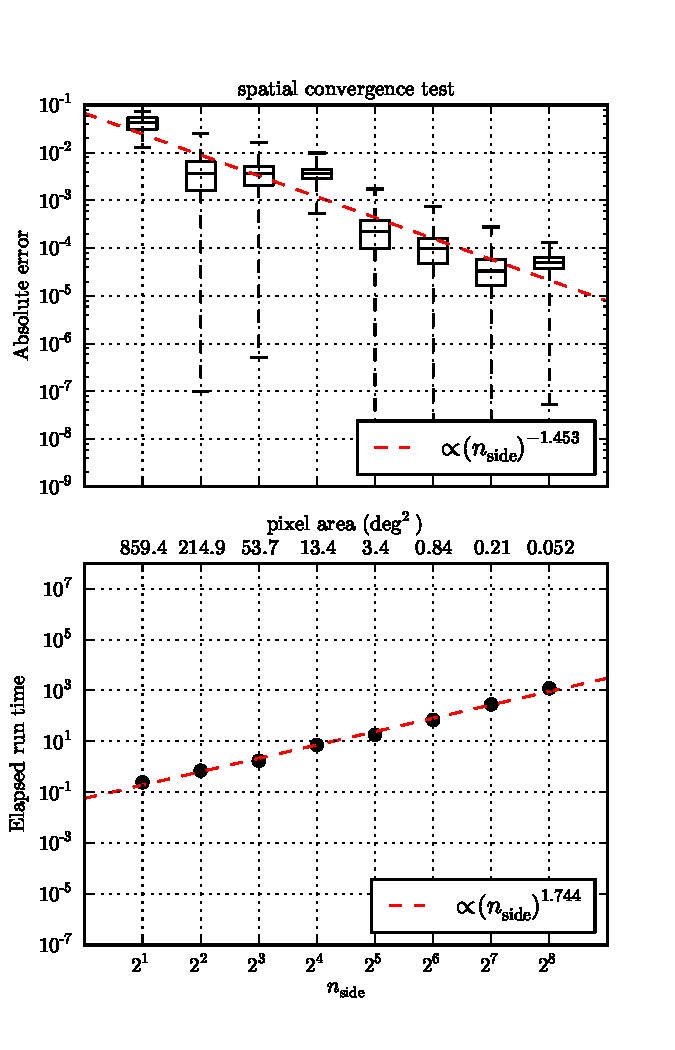
\includegraphics[width=0.5\textwidth]{spatial}
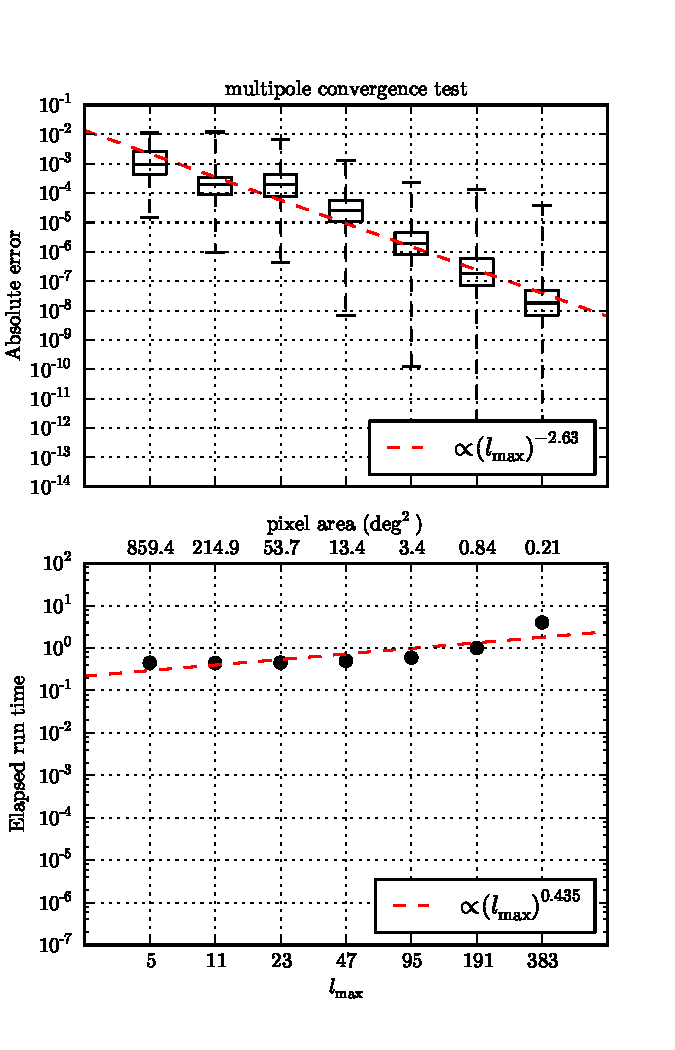
\includegraphics[width=0.5\textwidth]{multipole}
\end{staticcontents*}

\begin{staticcontents*}{healpix-dots}
\centering
figure 6d of~\citet{healpix}\\\vspace{5mm}
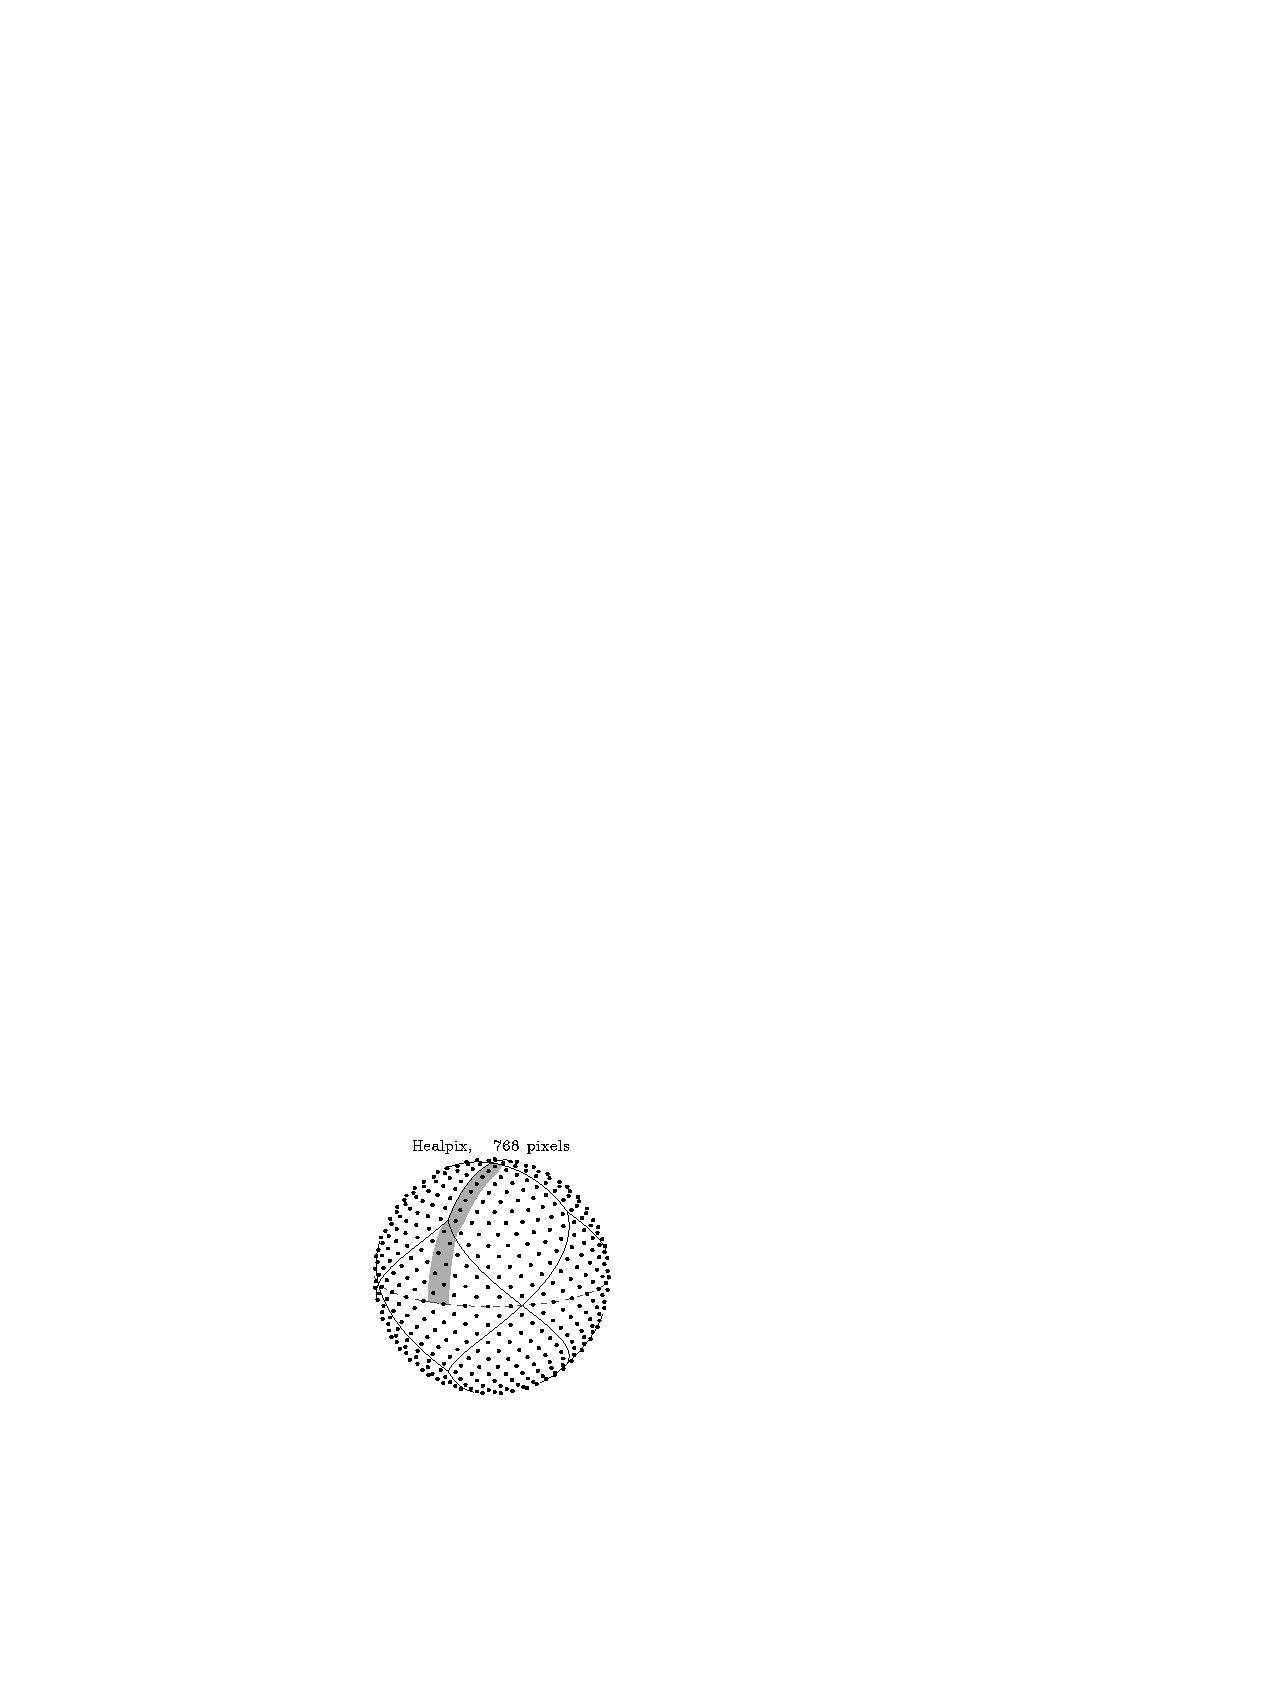
\includegraphics[width=\textwidth]{healpix-dots}
\end{staticcontents*}

\begin{staticcontents*}{ligosmile}
\begin{tabular}{ccccc}
	\begin{minipage}[c]{8cm}
		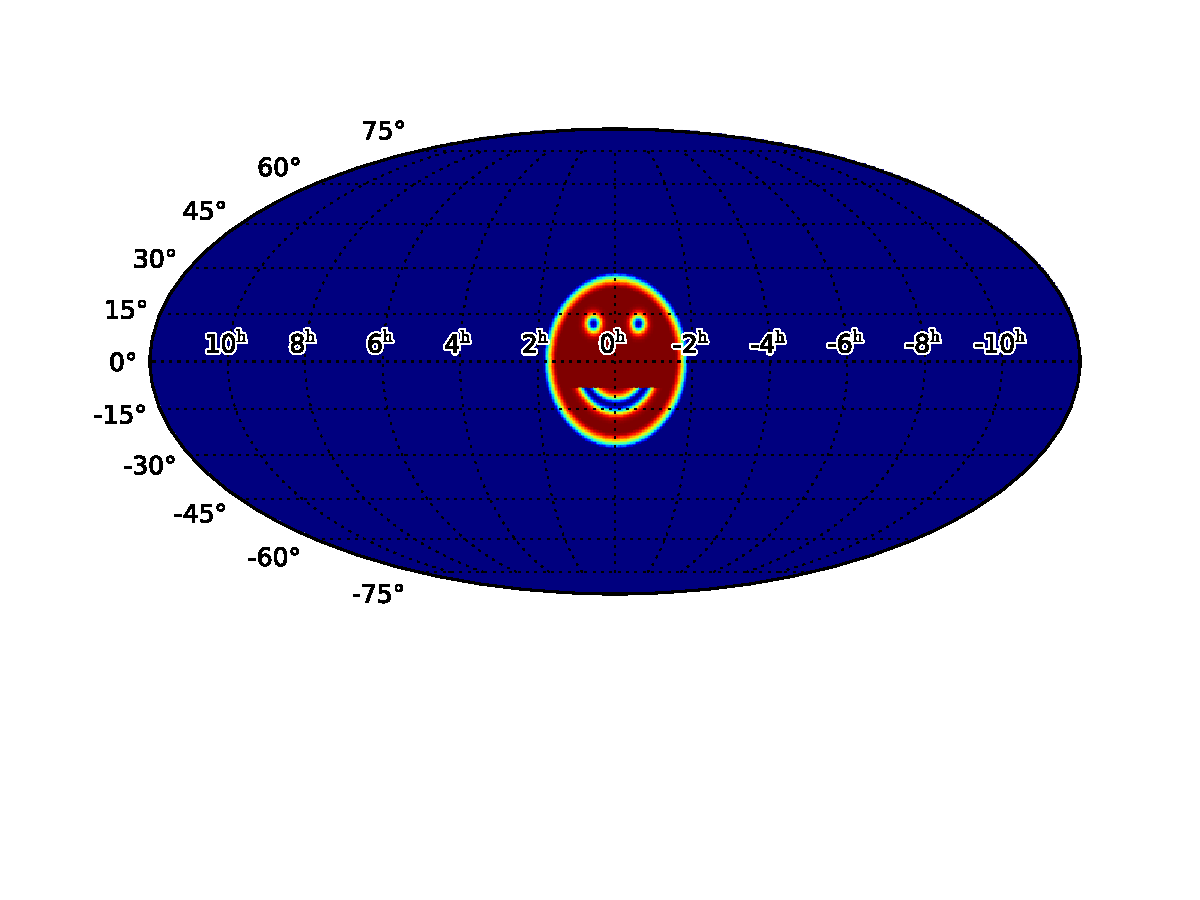
\includegraphics[width=\textwidth]{smile}
	\end{minipage} &
	{\Large$\star$} &
	\begin{minipage}[c]{8cm}
		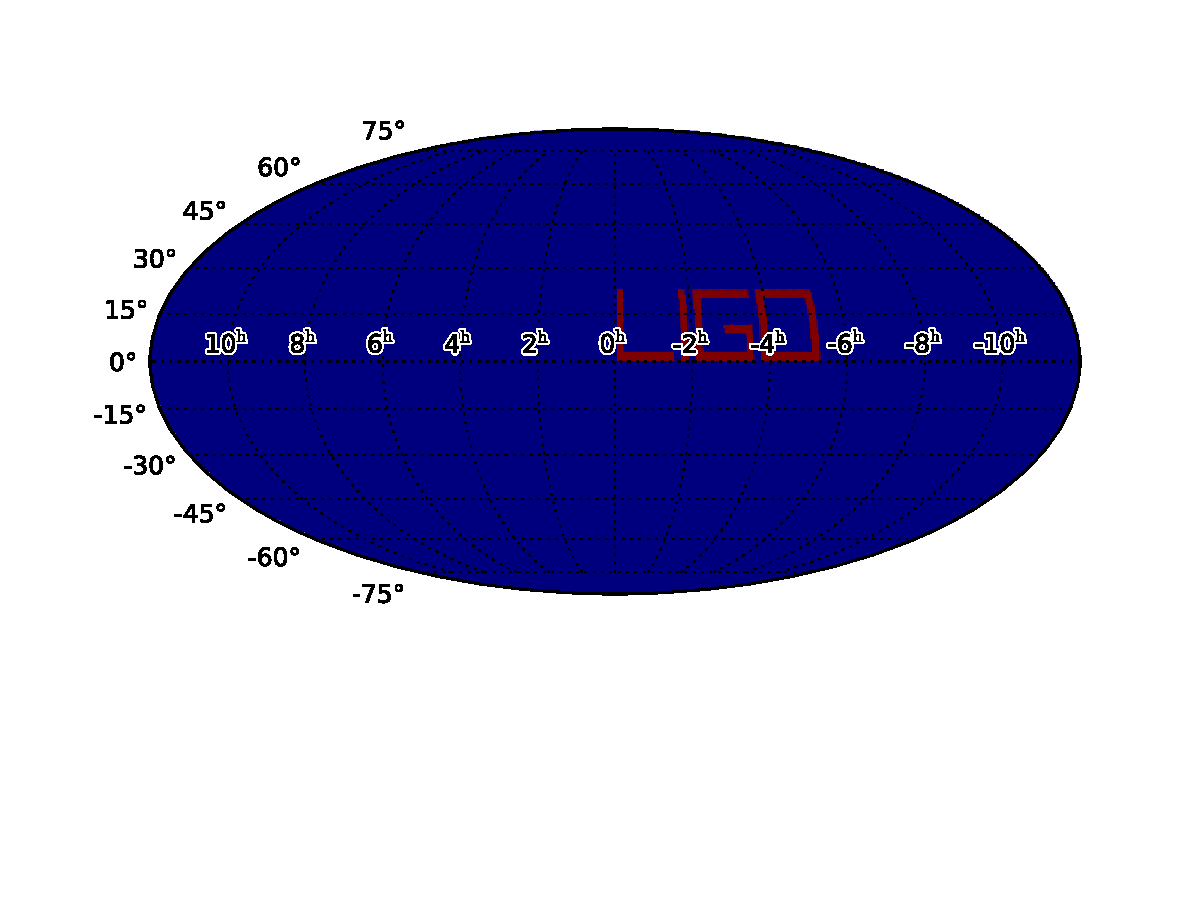
\includegraphics[width=\textwidth]{ligo}
	\end{minipage} &
	{\Large$=$} &
	\begin{minipage}[c]{8cm}
		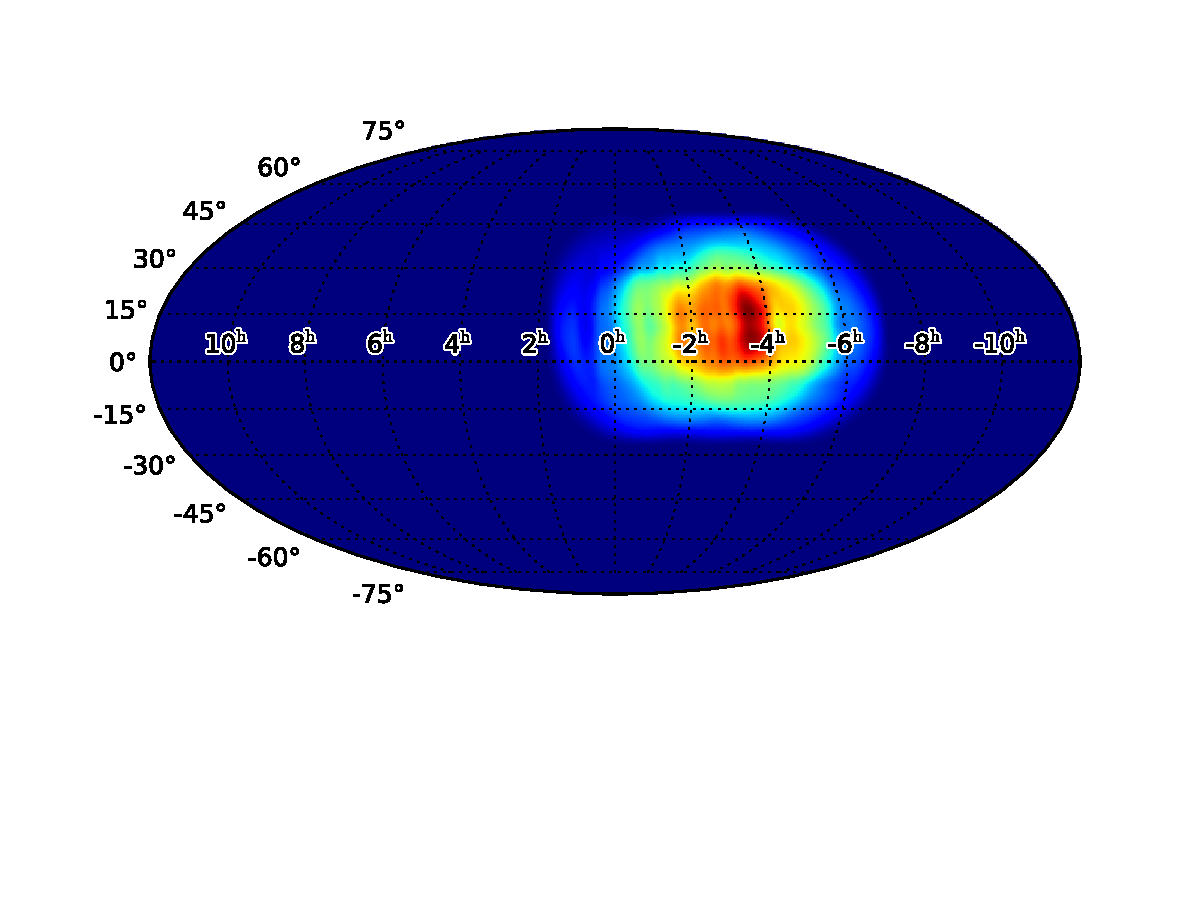
\includegraphics[width=\textwidth]{ligosmile}
	\end{minipage} \\
	{\fontspec{Marvel Bold}\large Field of view} &
	&
	{\fontspec{Marvel Bold}\large GW sky map} &
	&
	{\fontspec{Marvel Bold}\large Cross-correlation}
\end{tabular}
\end{staticcontents*}

\begin{staticcontents*}{flowchart}
\pgfdeclarelayer{background layer}
\pgfdeclarelayer{foreground layer}
\pgfsetlayers{background layer,foreground layer}
\begin{tikzpicture}
	\begin{pgfonlayer}{foreground layer}
	\matrix (m) [
		matrix of nodes,
		row sep=2cm,
		every node/.style={fill=white, inner sep=0.75cm, anchor=center, align=center},
		every path/.style={line width=4pt}
	] {
		\node[draw, shape=rounded rectangle, text width=6cm] (1) {Begin}; \\
		\node[draw, shape=rectangle, text width=6cm] (2) {Read next telescope's FOV}; \\
		\node[draw, shape=rectangle, text width=10cm] (3) {Mask out parts of sky that are in daytime or twilight}; \\
		\node[draw, shape=rectangle, text width=6cm] (4) {Convolve FOV with skymap}; \\
		\node[draw, shape=rectangle, text width=6cm] (5) {Locate maximum}; & \node[draw, shape=starburst, random starburst=12, starburst point height=1.5cm] (55) {to telescope}; \\
		\node[draw, shape=rectangle, text width=6cm] (6) {Mask out FOV from skymap}; \\
		\node[draw, shape=diamond, aspect=2, text width=6cm] (7) {Any telescopes left?}; \\
		\node[draw, shape=rounded rectangle] (8) {Done}; \\
	};
	\end{pgfonlayer}
	\begin{pgfonlayer}{background layer}
	\draw[line width=4pt, ->] (1) -- (2);
	\draw[line width=4pt, ->] (2) -- (3);
	\draw[line width=4pt, ->] (3) -- (4);
	\draw[line width=4pt, ->] (4) -- (5);
	\draw[line width=4pt, ->] (5) -- (6);
	\draw[line width=4pt, ->] (6) -- (7);
	\draw[line width=4pt, line cap=rect, ->] (7) -- (8) node[very near start, right] {no};
	\draw[line width=4pt, ->] (5) -- (55);
	\draw[line width=4pt, line cap=rect] (7) -| ($(55.south)+(-2cm,-0.5cm)$) node[at start, above] {yes};
	\draw[line width=4pt, ->] ($(55.north)+(-2cm,0.5cm)$) |- (2);
	\end{pgfonlayer}
\end{tikzpicture}
\end{staticcontents*}

\dropcap{P}{lanning} optical followup of gravitational wave (GW) events is a challenging optimization problem.  GW sky maps are multimodal and dispersed over 4π.  A telescope’s field of view (FOV) may have gaps between CCDs, dead CCDs, or vignetted or clipped regions.  Any of these complications make it difficult to decide on the “best” place to point a telescope.

We realized that if we phrased the single telescope problem as a cross-correlation of the telescope’s FOV and the GW sky map, we could attack it with \emph{HEALPix} --- the workhorse of CMB maps --- and spherical harmonic analysis.

Our summer student (A. Speranza) implemented the fast convolution of~\citet{Wandelt:2001p13439} and used it to compute the probability of imaging an EM counterpart.  As we expected, the harmonic analysis algorithm was much faster than the spatial algorithm.

What surprised us was that coordinating all of the observations by maximizing the probability of imaging the source conditioned on all of the telescopes’ pointings \emph{doubled} the number of detectable sources as compared to deciding each telescope’s configuration in isolation.

\framebreak

\parshape 2 0cm 19cm 0cm 27cm
Our key results are the two figures below.  At left is the fraction of injected signals that we would have imaged with one pointing of each telescope at the time of the trigger as a function of luminosity distance.  Solid lines represent observing plans that account for interference from the Sun and Earth.  Dashed lines represent observing plans in which these considerations are neglected.

We tested three different planning algorithms:

\paragraph{\color{red}noncooperative}
Each telescope is independently pointed where it is most likely to observe an EM counterpart.

\paragraph{\color{green!50!black}greedy sorted}
Suppose that we have chosen pointings for telescopes 1, 2, $\dots$, $i$.  The pointing of telescope $i+1$ is chosen to maximize the probability of detection, subject to telescopes 1, 2, $\dots$, $i$, remaining fixed.

\paragraph{\color{blue}anneal}
Uses simulated annealing to the probability of imaging the source by varying the configurations of all of the telescopes simultaneously.

\section*{Single telescope case}

\dropcap{T}{he} posterior distribution of source location $\omega$ given all GW observations \GW\ is commonly called the GW sky map, denoted $p(\omega | \GW)$.

Let $\EM{i}$ denote the event of observing an optical transient with telescope $i$.  Let $\gamma_i$ represent the pointing of telescope $i$.  The probability of observing an EM counterpart in telescope $i$ given its pointing $\gamma_i$ is
%
$$
	p(\EM{i} | \gamma_i, \omega) \equiv b_i(\gamma_i^{-1} \omega) \, v_i(\omega).
$$
%
Here, the function $b_i(\gamma_i^{-1} \omega)$ describes the telescope's (rotated) FOV and $v_i$ describes environmental features such as the twilight/nighttime terminator, the horizon, and optionally the seeing.
%
Now, marginalizing over the unknown source location, this becomes
%
\begin{equation}
	\label{eq:single-telescope-integral}
	p(\EM{i} | \gamma_i, \GW) \equiv \int b_i(\gamma_i^{-1} \omega) \, v(\omega) \, s(\omega) \, \mathrm{d}\Omega.
\end{equation}
%
The optimal pointing is
%
$$
	\gamma_i^* \equiv \arg \max_{\gamma_i} p(\EM{i} | \gamma_i, \GW).
$$

\framebreak

\section*{\hspace{3cm}Numerical implementation}

\parshape 8
	4.25cm 22.75cm
	4.5cm 22.5cm
	4.75cm 22.25cm
	4.5cm 22.5cm
	4.25cm 22.75cm
	4cm 23cm
	3.25cm 23.75cm
	0cm 27cm  
Equation~(\ref{eq:single-telescope-integral}) resembles a cross-correlation integral.  For scalar functions, the convolution theorem and the fast Fourier transform (FFT) make cross-correlation in the frequency domain very efficient.  \citet{Driscoll1994202}, \citet{Wandelt:2001p13439}, and others have described analogous fast convolution algorithms for functions defined on the unit sphere.  We used \emph{HEALPix} to write two convolution algorithms:

\paragraph{spatial}
uses nearest neighbor interpolation of the rotated kernel to approximate the integral in spherical polar coordinates.

\paragraph{multipole}
involves a spherical harmonic transform of both the masked sky map $v_i(\omega)s(\omega)$ and the FOV $b_i(\omega)$, a weighted inner product of the spherical harmonic coefficients, and a 2D inverse FFT to return to polar coordinates.\\

We checked convergence and run time of both algorithms.  At a resolution of $\approx$~0.05~deg$^\mathsf{2}$, \textbf{spatial} takes $\approx$1000~s while \textbf{multipole} takes $\approx$25~s of CPU time.  Both versions are \emph{OpenMP} accelelerated to exploit multiple cores.  On the LIGO-Caltech cluster head node, the \textbf{multipole} algorithm has achieved run times as short as 5~s, though further speedup is possible.

\vspace{1cm}
\makebox[25cm][r]{\raggedleft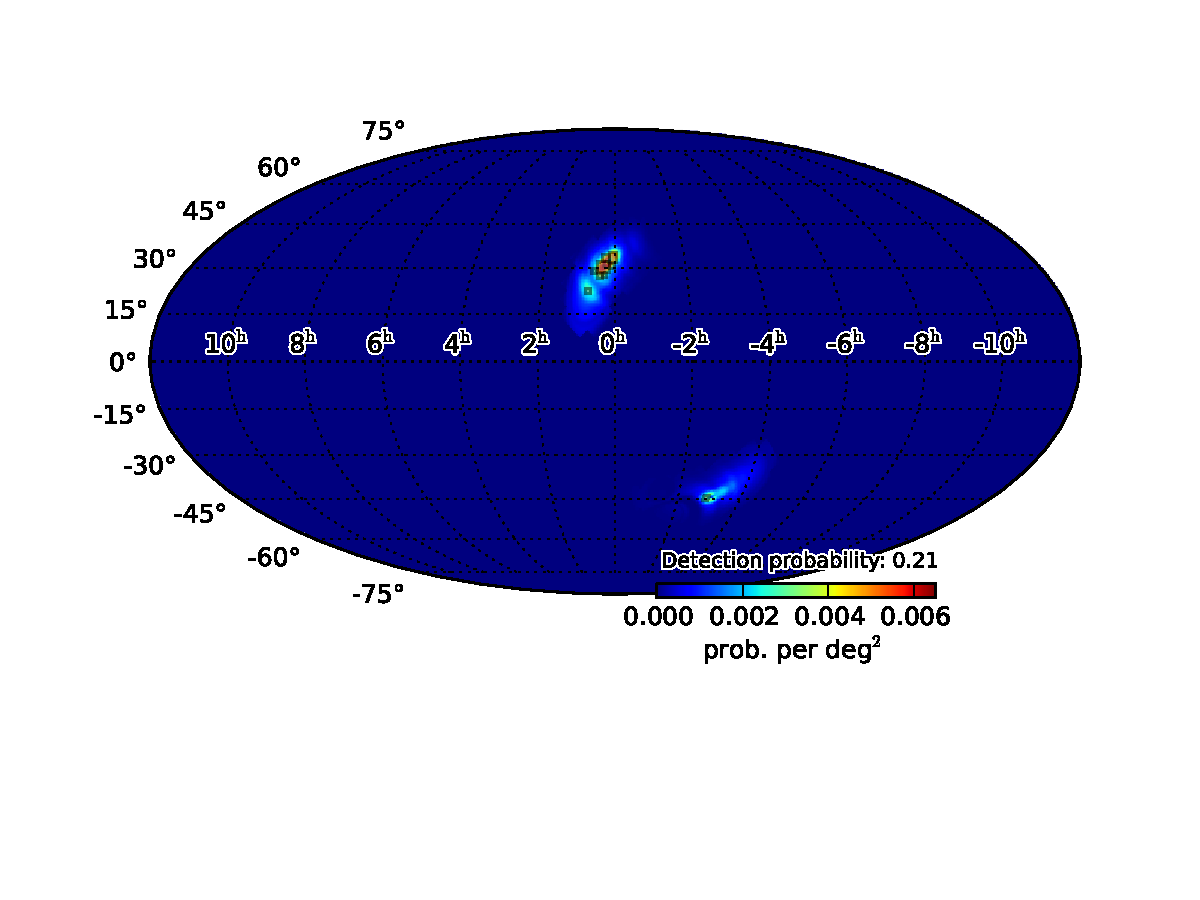
\includegraphics[width=26cm]{example-no-interference}}

%\framebreak
\begin{staticcontents*}{spilled-text}
\section*{Multiple telescope case}

\dropcap{F}{or} multiple telescopes, the figure of merit is the probability of imaging the source with at least one telescope:
%
\begin{align}
	\label{eq:p_any}
	p_{\geqslant 1} \equiv p(\EM{1} \cup \EM{2} \cup \dots \cup \EM{N} | \gamma_1, \gamma_2, \dots, \gamma_N, \GW) \nonumber \\
	= 1 - \int
		\left[ 1 - b_1 \left( \gamma_1^{-1} \omega \right) v_1(\omega) \right]
		\left[ 1 - b_2 \left( \gamma_2^{-1} \omega \right) v_2(\omega) \right] \nonumber \\ \cdots
		\left[ 1 - b_N \left( \gamma_N^{-1} \omega \right) v_N(\omega) \right]
		s(\omega) \, \mathrm{d}\Omega.
\end{align}
%
The integral expression above can be evaluated iteratively one telescope at a time, suggesting a greedy algorithm depicted in the flow chart at right.

The most sophisticated planning algorithm that we tried used simulated annealing to simultaneously vary the pointings of all of the telescopes.  We used the Python module \texttt{scipy.optimize.anneal} and a modified version of the ``very fast'' cooling schedule described by \citet{Ingber1989967}.

\section*{Case study}

We compared the detection efficiency of the noncoordinated planner and our two coordinated planners using a set of 2126 GW skymaps from low-mass inspiral signals injected into 24 hours of simulated initial LIGO noise.

\hspace{2em}We computed the environmental masks $v_i(\omega)$ using the Python edition of \emph{NOVAS}, the US Naval Observatory's positional astronomy library.

\hspace{2em}Surprisingly, we found that (a) \textit{greedy} performed almost as well as \emph{anneal} in terms of detection efficiency, and (b) both coordinated planners had roughly \emph{double} the detection efficiency of the \emph{noncoordinated} planner.
\end{staticcontents*}

\framebreak

\section*{Conclusion}

\dropcap{W}{e} have demonstrated that coordinating observations amongst multiple telescopes is a promising strategy for EM followup of GW events.  We have developed an observation planning code that is \emph{fast} enough to be used for extensive simulation campaigns and \emph{flexible} enough to accommodate any network of telescopes.  Our code aims to be \emph{scalable} enough to produce observing plans in near real-time on a multi-core machine.

This project lays the groundwork for future multi-messenger studies that will account for a mix of telescopes with different limiting magnitudes, slew times, in addition to fields of view.

\bibliographystyle{apj}
\bibliography{../bayestar-paper/proposal,../bayestar-paper/telescope,../bayestar-paper/telescope_list}
\noindent
http://aa.usno.navy.mil/software/novas

\noindent\\
LIGO was constructed by the California Institute of Technology and Massachusetts Institute of Technology with funding from the National Science Foundation (NSF) and operates under cooperative agreement PHY-0107417.  This research is supported by NSF through a Graduate Research Fellowship to LS.  This poster has LIGO Document Number LIGO-G1100983-v4.

\end{document}
